\section{The Mokaminter App}\label{sec:mokaminter}

We have developed the Mokaminter app for mining with proof of space.
It creates and maintains a list of remote miners, each connected
to a peer of the same or of different blockchains.
Mokaminter is an open-source app for Android, distributed
on Google Play~\cite{mokaminter-google-play} under
the Apache 2.0 license. Its source code is available at~\cite{mokaminter-source-code}.
An iPhone version might be eventually available,
but it is more difficult to build since
it cannot leverage existing Java libraries from desktop miners.

Mokaminter works for blockchains built through
the Mokamint generic engine~\cite{mokamint-source-code} (see Fig.~\ref{fig:mining}), that implements
the proof of space algorithm in~\cite{Spoto25}. Mokamint
implements the networking and consensus layers of
a blockchain, while the application layer is left generic and can be built on top.
This idea of a pluggable application layer has been borrowed from Tendermint~\cite{Kwon14}.
Currently, there exist Mokamint applications for Hotmoka~\cite{hotmoka}, a software layer
for running Solidity-like smart contracts in a subset of Java~\cite{Spoto19}, and
for a ledger functionally
equivalent to Bitcoin~\cite{bitcoin-mokamint}. Therefore Mokaminter mines, at the moment,
for either of those blockchains, with more to come in the future.

Creation and activation of a miner works as follows:
(1) the user specifies the URI (universal resource identifier) of a
blockchain peer running Mokamint and the desired number of nonces for the plot file;
  %(Fig.~\ref{fig:mokaminter_add_miner}, above);
(2) the app creates a new private/public key pair to identify the miner,
  represented, as usual from Bitcoin's time~\cite{Antonopoulos23},
  in terms of a $12$ words mnemonics; % (Fig.~\ref{fig:mokaminter_add_miner}, below);
  alternatively, the user can insert the $12$ words of an existing key pair;
(3) the app informs the user about the expected size of the plot file
  and asks for confirmation; % (Fig.~\ref{fig:mokaminter_confirmation});
(4) if confirmed, the plot file gets created in the background;
(5) once the plot is created, the app adds a miner tile
  and activates a background process that mines by using the new plot.
  %(Fig.~\ref{fig:mokaminter_mining}).

%\begin{figure}[t]
%  \begin{center}
%    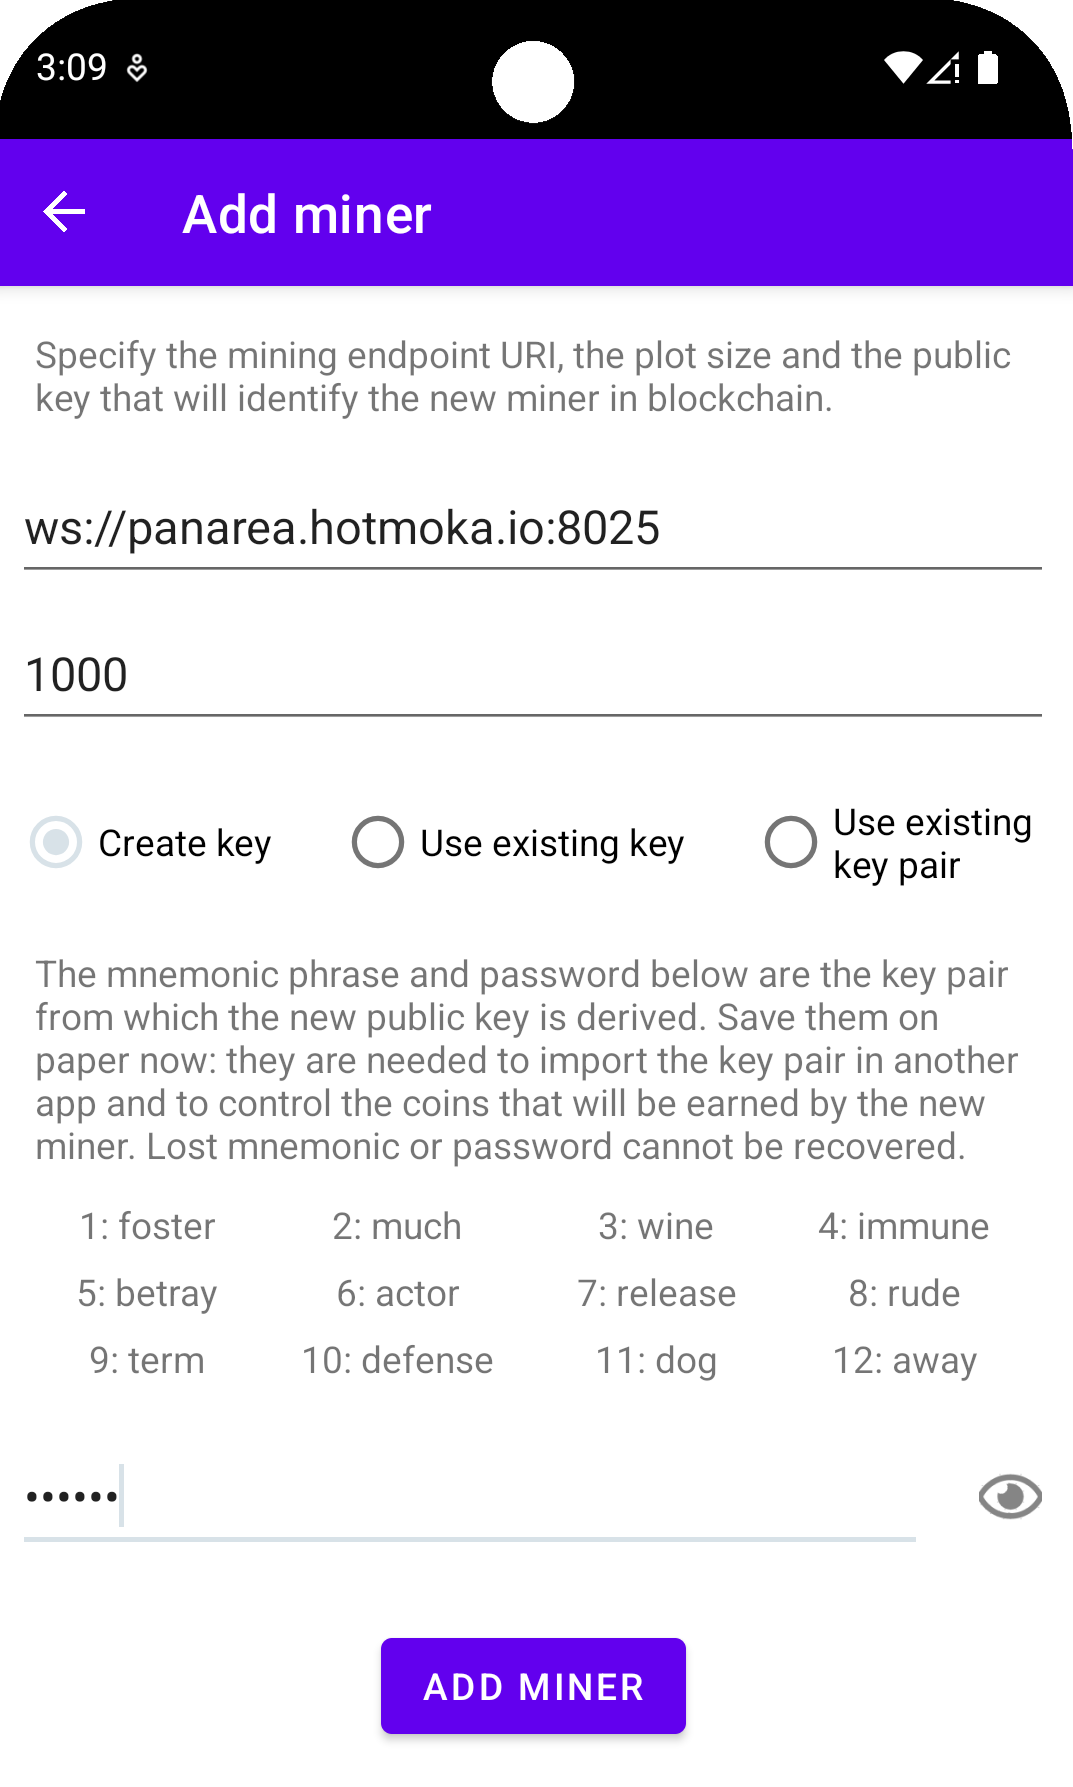
\includegraphics[width=\textwidth/3]{pictures/mokaminter_add_miner}
%  \end{center}
%  \caption{Specification of the parameters for the creation of a miner.}
%  \label{fig:mokaminter_add_miner}
%\end{figure}

%\begin{figure}[b]
%  \begin{center}
%    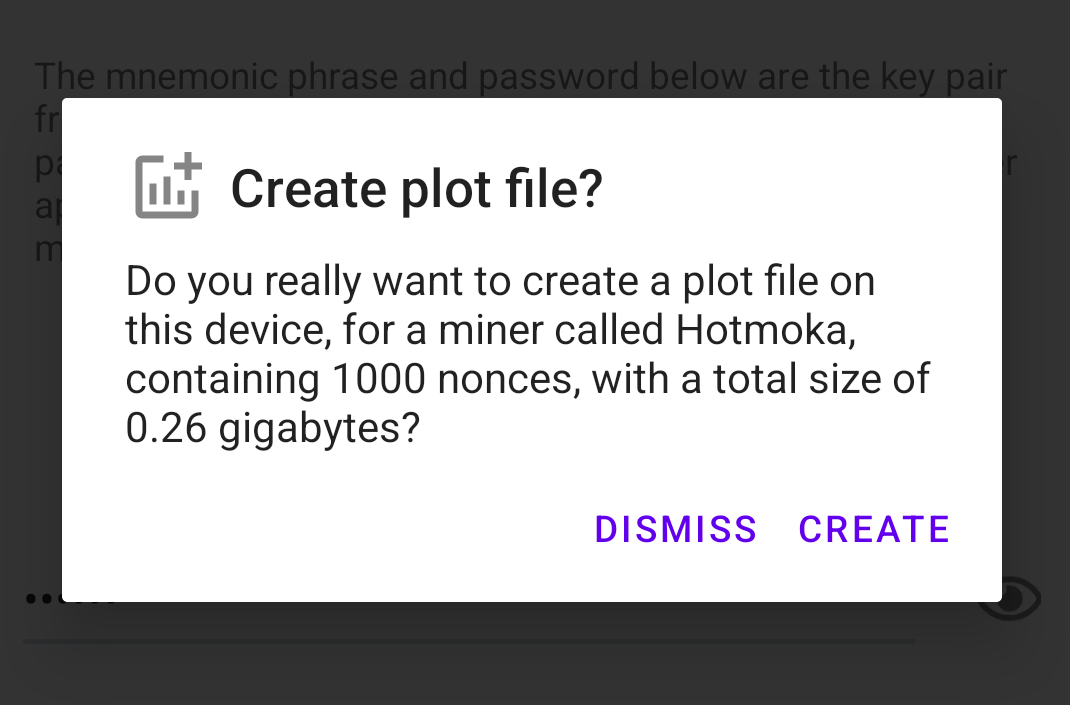
\includegraphics[width=\textwidth/3]{pictures/mokaminter_confirmation}
%  \end{center}
%  \caption{Confirmation is required before creating a new plot file.}
%  \label{fig:mokaminter_confirmation}
%\end{figure}

%\begin{figure}[t]
%  \begin{center}
%    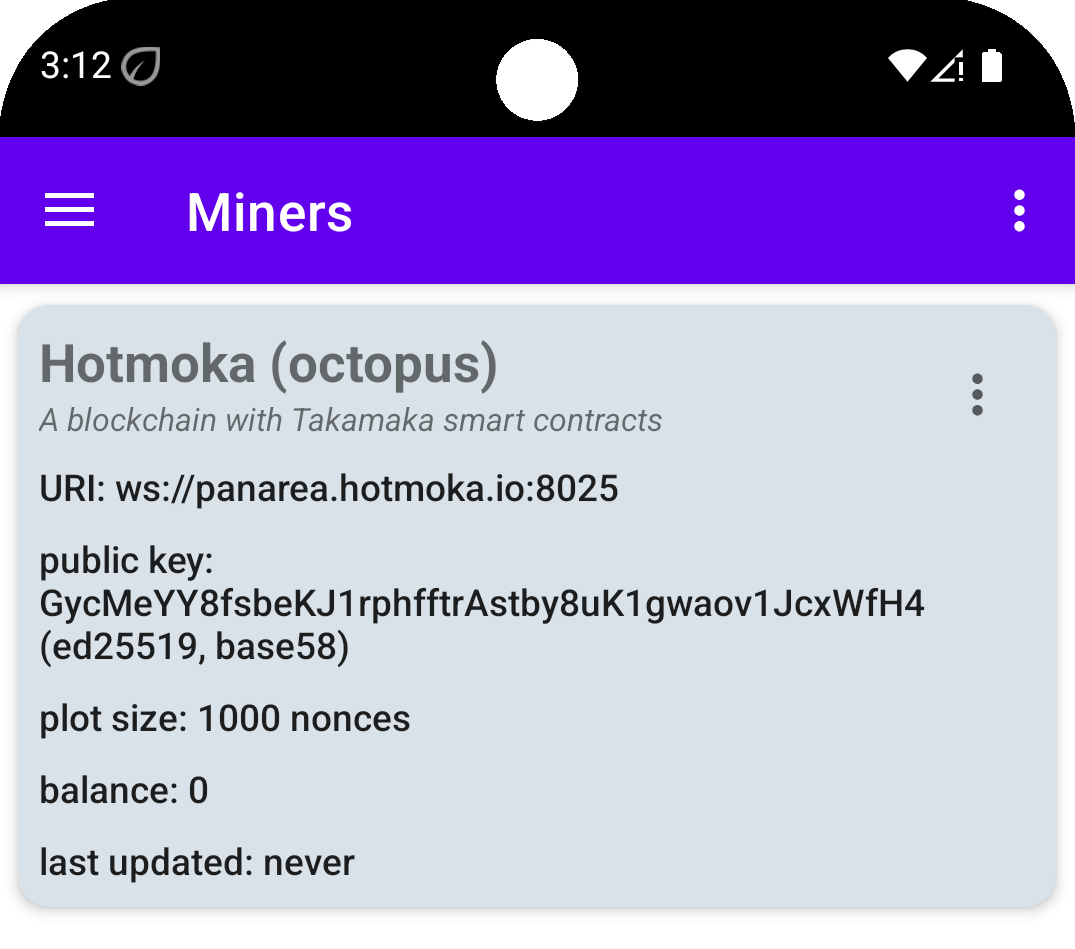
\includegraphics[width=\textwidth/3]{pictures/mokaminter_mining}
%  \end{center}
%  \caption{A new tile for a miner, working in the background. Eventually, its
%  cryptocurrency balance will increase.}
%  \label{fig:mokaminter_mining}
%\end{figure}

\vspace{0.5ex}\noindent\textbf{Security considerations.}
%
A lost or stolen device is a relatively frequent event.
If private keys were kept in the device, who finds
or steals the device could also steal the cryptocurrency accumulated while mining with such keys.
Therefore, Mokaminter does not store private keys.
Namely, only the public key is needed to create the plot (Def.~\ref{def:nonce_construction}), and
the app can forget the private key. This entails, however,
that the user must not lose the $12$ words of the key pair,
or otherwise the earned crypto becomes inaccessible.
The use of the miner's \emph{public} key for the construction of its nonces
(step.~\ref{step:nonce_construction:seed}
of Def.~\ref{def:nonce_construction}) might seem
to be a security issue, since anyone can impersonate a miner.
But that impersonation could only be a help for the impersonated miner:
the impersonator might create nonces that are so good to win
the mining competition, whose reward will go to the public key (hence to the miner);
or nonces that lose the mining competition, in which case they are just ignored;
or syntactically illegal nonces, in which case Mokamint bans the IP of the impersonator
(it does not ban the public key of the miner). In any case, the impersonated miner
can only win from the impersonation.

\vspace{0.5ex}\noindent\textbf{Usability considerations.}
%
A mobile app has quite different usability considerations than a desktop application.
A first one is about feedback.
A desktop user can check warnings, error messages and logs.
In a mobile app, this is possible
but uncomfortable for most users. Therefore, Mokaminter gives feedback through
a heartbeat effect at each challenge, to inform the user that it is
actually mining. Moreover, network disconnection
turns the miner's tile gray in the list of miners.
%
Another usability issue is related to the insertion of the
$12$ words, to import an existing key pair.
This is frustrating and error-prone with the software keyboard of a mobile device.
Thus, Mokaminter autocompletes words while typing.
%
A last issue is the risk of specifying a plot dimension that is
too large to complete the plot's creation in a reasonable time:
this would hang the device and drain its battery. To avoid this risk,
Mokaminter imposes a maximum plot dimension, that the user can override
with an explicit decision.

\vspace{0.5ex}\noindent\textbf{Technical considerations.}
%
Mokaminter uses websockets for network connections,
that perfectly match the continuous, bidirectional flow of challenges
and answers (Fig.~\ref{fig:mining}). But network connection in a
mobile device may be relatively unstable (thick walls, tunnels, network switches).
Mokaminter tries to reconnect if the connection is lost or
if it has not received any challenge for some time. If reconnection fails, it
tries again after a minute, to avoid draining the battery with too
frequent attempts. Background mining execution and battery optimization
are a complication solved through the official
Android good practice~\cite{background-tasks}
that ensures a background task to run continously,
leveraging either a \texttt{WorkManager} or a \texttt{JobService}, depending on the
Android version, together with a foreground notification.
%
%Another technical issue is related to the background task for mining.
%The Android system is extremely restrictive with background
%tasks, since they might drain the battery. There are official guidelines
%for them, but they changed across different Android versions and
%phone manufacturers often add extra constraints. Many phones
%turn Mokaminter off overnight, when
%the Android system enters a special \emph{doze mode}. If this happens, it is enough
%for the user
%to turn it on again in the morning. A better solution does not seem in sight, at the moment.

